
\chapter{Ethical Approval}\label{ch:Ethical Approval}

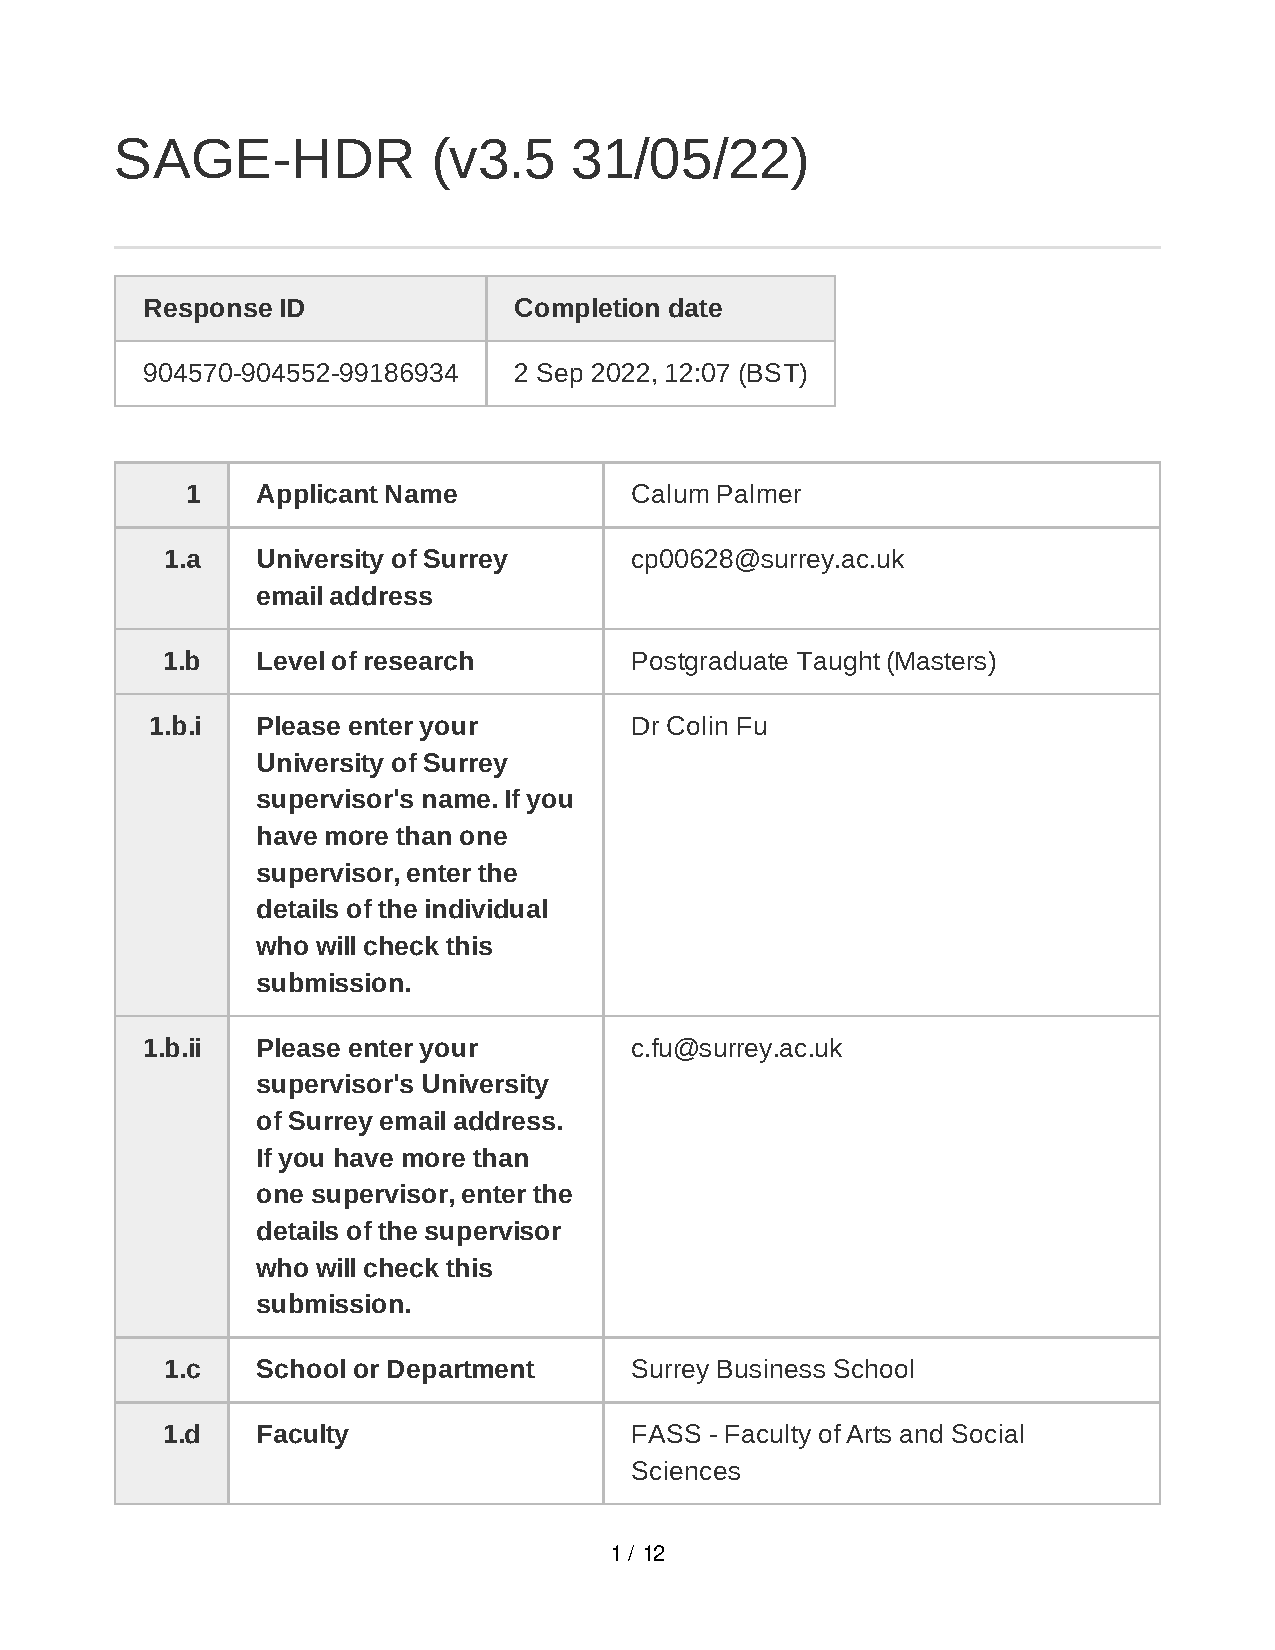
\includepdf[pages=-]{EthicForm.pdf}

\chapter{Python Code}\label{ch:Python Code}

\begin{lstlisting}[language=python,label={lst:pythoncode}]
import pandas as pd
import numpy as np
import matplotlib.pyplot as plt
import seaborn as sns
from scipy import stats
import jinja2
from pycaret.classification import *
from pycaret.utils import check_metric
SEED = 123

# DATA INPUT AND CLEANING
# 123 Columns and 150k rows means that the data needs to be simplified and the non-essentials be stripped.
df = pd.read_csv("2021_LoL_esports_match_data_from_OraclesElixir_20220606.csv")
df_copy = df.copy()
df.shape

# Filtering for completed data, team data and removing features that are non-team related or deemed useless for our model
df = df[df["datacompleteness"] == "complete"]
df = df[df["position"] == "team"]
df = df.drop_duplicates(subset = "gameid")
col_drop = ["url", "year", "split", "date", "game", "participantid", "playername", "playerid", "teamid", "champion",
            "ban1", "ban2", "ban3", "ban4", "ban5", "kills", "deaths", "assists", "teamkills", "teamdeaths",
            "doublekills", "triplekills", "quadrakills", "pentakills", "firstbloodkill", "firstbloodassist",
            "firstbloodvictim", "team kpm", "ckpm", "dragons", "opp_dragons", "elementaldrakes", "opp_elementaldrakes",
            "infernals", "mountains", "clouds", "oceans", "chemtechs", "hextechs", "dragons (type unknown)",
            "elders", "opp_elders", "heralds", "opp_heralds", "barons", "opp_barons", "towers", "opp_towers",
            "turretplates", "opp_turretplates", "inhibitors", "opp_inhibitors", "damagetochampions", "dpm",
            "damageshare", "damagetakenperminute", "damagemitigatedperminute", "wardsplaced", "wpm", "wardskilled",
            "wcpm", "controlwardsbought", "visionscore", "vspm", "totalgold", "earnedgold", "earned gpm",
            "earnedgoldshare", "goldspent", "gspd", "total cs", "minionkills", "monsterkills", "monsterkillsownjungle",
            "monsterkillsenemyjungle", "cspm", "opp_goldat10", "opp_goldat15", "goldat10", "goldat15", "csat10",
            "csat15", "opp_csat10", "opp_csat15", "xpat10", "xpat15", "opp_xpat10", "opp_xpat15", "league",
            "opp_assistsat10", "opp_killsat10", "opp_assistsat15", "opp_killsat15", "opp_deathsat10", "opp_deathsat15",
            "gameid", "datacompleteness", "teamname", "side", "position",]
df.drop(col_drop, inplace=True, axis=1)
df = df.dropna()
df_copy = df.copy()

# Correlation of the features is then completed
# If we consider a Correlation of 0.5 or above to be a 'Strong' correlation
plt.figure(figsize=(18, 16))
mask = np.zeros_like(df.corr(), dtype=np.bool)
mask[np.triu_indices_from(mask)] = True
cmap = sns.diverging_palette(10, 250, as_cmap=True)
sns.heatmap(df.corr(method="kendall"), cmap=cmap, annot=True, fmt='.2f', vmin=-1, vmax=1,
            mask = mask, square=True, linewidths=.8, center = 0)

# Reworking and dropping any strongly correlated features
df["KillParat10"] = df["assistsat10"] + df["killsat10"]
df["KillParat15"] = df["assistsat15"] + df["killsat15"]
df = df.drop(df[df.patch == 10.25].index)
df["patch"] = (df["patch"] - 11)*100
round(df["patch"], 1)
df_copy = df.copy()
feature_drop = ["assistsat10", "killsat10", "assistsat15", "killsat15", "golddiffat10", "golddiffat15",
                "xpdiffat10", "xpdiffat15",]
df = df.drop(feature_drop, axis=1)

plt.figure(figsize=(18, 16))
mask = np.zeros_like(df.corr(), dtype=np.bool)
mask[np.triu_indices_from(mask)] = True
cmap = sns.diverging_palette(10, 250, as_cmap=True)
sns.heatmap(df.corr(method="kendall"), cmap=cmap, annot=True, fmt='.2f', vmin=-1, vmax=1,
            mask = mask, square=True, linewidths=.8, center = 0)

# Descriptive statistics to find if there are any outliers
with pd.option_context('display.max_columns', 15):
    print(df.describe())

# Removing the outliers found in the high end of gamelength
df = df.loc[df["gamelength"] <= np.quantile(df["gamelength"], q=0.99)]
with pd.option_context("display.max_columns", 15):
    print(df.describe())

# Normalization
#from sklearn import preprocessing
#scaler = preprocessing.MinMaxScaler()
#names = df.columns
#d = scaler.fit_transform(df)
#scaled_df = pd.DataFrame(d, columns=names)
#df = scaled_df

from sklearn.feature_selection import RFE
from sklearn.tree import DecisionTreeClassifier
# define dataset
y = df.result
X = df.drop("result", axis=1)
# define RFE
rfe = RFE(estimator=DecisionTreeClassifier(), n_features_to_select=12)
# fit RFE
rfe.fit(X, y)
# summarize all features
for i in range(X.shape[1]):
    print('Column: %d, Selected %s, Rank: %.3f' % (i, rfe.support_[i], rfe.ranking_[i]))

# New correlation matrix with updated feature set
plt.figure(figsize=(18, 10))
mask = np.zeros_like(df.drop("result",axis=1).corr(), dtype=np.bool)
mask[np.triu_indices_from(mask)] = True
sns.heatmap(df.drop("result",axis=1).corr(), cmap=cmap, annot=True, fmt='.2f', vmin=-1, vmax=1,
            mask = mask, square=True, linewidths=.8, center = 0)
plt.title('Correlation Matrix between Features')

df = pd.DataFrame(data=df)

#  Split the data into separate 10 and 15 minute datasets
feature_drop2 = ["firstbaron", "firsttothreetowers"]
at10 = []
for column in list(df.columns):
    if '10' in column:
        at10.append(column)
at15 = []
for column in list(df.columns):
    if '15' in column:
        at15.append(column)
df10 = df.drop(at15, axis = 1)
df15 = df.drop(at10, axis = 1)
df20 = df.drop(at10, axis = 1)
df10.drop(feature_drop2, axis = 1, inplace=True)
df15.drop(feature_drop2, axis = 1, inplace=True)

# Correlation matrix of the 10 minute dataset
plt.figure(figsize=(12, 10))
mask = np.zeros_like(df10.drop("result",axis=1).corr(), dtype=np.bool)
mask[np.triu_indices_from(mask)] = True
sns.heatmap(df10.drop("result",axis=1).corr(), cmap=cmap, annot=True, fmt='.2f', vmin=-1, vmax=1,
            mask = mask, square=True, linewidths=.8, center = 0)
plt.title('Correlation Matrix between Features (10 minute dataset)')

# Correlation matrix of the 15 minute dataset
plt.figure(figsize=(12, 10))
mask = np.zeros_like(df15.drop("result",axis=1).corr(), dtype=np.bool)
mask[np.triu_indices_from(mask)] = True
sns.heatmap(df15.drop("result",axis=1).corr(), cmap=cmap, annot=True, fmt='.2f', vmin=-1, vmax=1,
            mask = mask, square=True, linewidths=.8, center = 0)
plt.title('Correlation Matrix between Features (15 minute dataset)')

# Correlation matrix of the 20 minute dataset
plt.figure(figsize=(12, 10))
mask = np.zeros_like(df20.drop("result",axis=1).corr(), dtype=np.bool)
mask[np.triu_indices_from(mask)] = True
sns.heatmap(df20.drop("result",axis=1).corr(), cmap=cmap, annot=True, fmt='.2f', vmin=-1, vmax=1,
            mask = mask, square=True, linewidths=.8, center = 0)
plt.title('Correlation Matrix between Features (20 minute dataset)')

# Now we check to see if the results are balanced
# Slightly skewed but is fine to use.
print("Blue side win rate: {0:.1f}%".format(df15["result"].sum() / df15["result"].shape[0]*100))
sns.set_style('whitegrid')
fig = sns.countplot(x= df15.result , data=df15, palette= "Blues")
fig.set(xlabel= "Result", ylabel= "Count of Matches", title = "Balance of the dataset")
fig.set_xticklabels(["Loss", "Win"]),

df15.hist(alpha = 0.9, figsize=(12,10), bins=20);

# Baseline Model for 10 minute data
from sklearn.ensemble import RandomForestClassifier
from sklearn.metrics import accuracy_score
from sklearn.model_selection import train_test_split

y = df10.result
X = df10.drop("result", axis=1)
train_X, val_X, train_y, val_y = train_test_split(X, y, random_state=SEED)
rf_model = RandomForestClassifier(random_state=SEED)
rf_model.fit(train_X, train_y)
pred = rf_model.predict(val_X)
score = accuracy_score(val_y, pred)
print('Accuracy: %.2f%%' %(score*100))

# Baseline Model for 15 minute data
y = df15.result
X = df15.drop("result", axis=1)
train_X, val_X, train_y, val_y = train_test_split(X, y, random_state=SEED)
rf_model = RandomForestClassifier(random_state=SEED)
rf_model.fit(train_X, train_y)
pred = rf_model.predict(val_X)
score = accuracy_score(val_y, pred)
print('Accuracy: %.2f%%' %(score*100))

# Baseline Model for 20 minute data
y = df20.result
X = df20.drop("result", axis=1)
train_X, val_X, train_y, val_y = train_test_split(X, y, random_state=SEED)
rf_model = RandomForestClassifier(random_state=SEED)
rf_model.fit(train_X, train_y)
pred = rf_model.predict(val_X)
score = accuracy_score(val_y, pred)
print('Accuracy: %.2f%%' %(score*100))

# Building a model based on data from the 10 minute mark
models=setup(data=df10,
             target="result",
             silent=True,
             session_id=33,
            normalize=True,
            normalize_method="minmax")
# Comparing the different model's final results
model_results=compare_models()
model_results
lr_model=create_model('lr')
lr_tunedmodel=tune_model(lr_model)
plot_model(lr_tunedmodel, plot = 'auc')
plot_model(lr_tunedmodel, plot='feature')
plot_model(lr_tunedmodel, plot = 'confusion_matrix')
predict_model(lr_tunedmodel)
final_lr = finalize_model(lr_tunedmodel)
print(final_lr)
predict_model(final_lr)

df22 = pd.read_csv("2022_LoL_esports_match_data_from_OraclesElixir_20220606.csv")
df22.head

# Cleaning data on 2022 data
def data_clean(df):
    df = df[df["datacompleteness"] == "complete"]
    df = df[df["position"] == "team"]
    df = df.drop_duplicates(subset = "gameid")
    col_drop = ["url", "year", "split", "date", "game", "participantid", "playername", "playerid", "teamid", "champion",
            "ban1", "ban2", "ban3", "ban4", "ban5", "kills", "deaths", "assists", "teamkills", "teamdeaths",
            "doublekills", "triplekills", "quadrakills", "pentakills", "firstbloodkill", "firstbloodassist",
            "firstbloodvictim", "team kpm", "ckpm", "dragons", "opp_dragons", "elementaldrakes", "opp_elementaldrakes",
            "infernals", "mountains", "clouds", "oceans", "chemtechs", "hextechs", "dragons (type unknown)",
            "elders", "opp_elders", "heralds", "opp_heralds", "barons", "opp_barons", "towers", "opp_towers",
            "turretplates", "opp_turretplates", "inhibitors", "opp_inhibitors", "damagetochampions", "dpm",
            "damageshare", "damagetakenperminute", "damagemitigatedperminute", "wardsplaced", "wpm", "wardskilled",
            "wcpm", "controlwardsbought", "visionscore", "vspm", "totalgold", "earnedgold", "earned gpm",
            "earnedgoldshare", "goldspent", "gspd", "total cs", "minionkills", "monsterkills", "monsterkillsownjungle",
            "monsterkillsenemyjungle", "cspm", "opp_goldat10", "opp_goldat15", "goldat10", "goldat15", "csat10",
            "csat15", "opp_csat10", "opp_csat15", "xpat10", "xpat15", "opp_xpat10", "opp_xpat15", "league",
            "opp_assistsat10", "opp_killsat10", "opp_assistsat15", "opp_killsat15", "opp_deathsat10", "opp_deathsat15",
            "gameid", "datacompleteness", "teamname", "side", "position",]
    df.drop(col_drop, inplace=True, axis=1)
    df = df.dropna()
    df_NO = df.copy()
    df["KillParat10"] = df["assistsat10"] + df["killsat10"]
    df["KillParat15"] = df["assistsat15"] + df["killsat15"]
    feature_drop = ["assistsat10", "killsat10", "assistsat15", "killsat15", "golddiffat10", "golddiffat15", "xpdiffat10", "xpdiffat15"]
    df = df.drop(feature_drop, axis=1)
    df["patch"] = (df["patch"] - 12)*100
    round(df["patch"], 1)
    return df

df22 = data_clean(df22)
df22.describe

#  Split the data into separate 10 and 15 minute datasets
def data_split(df):
    feature_drop2 = ["firstbaron", "firsttothreetowers"]
    at10 = []
    for column in list(df.columns):
        if '10' in column:
            at10.append(column)
    at15 = []
    for column in list(df.columns):
        if '15' in column:
            at15.append(column)
    df10 = df.drop(at15, axis = 1)
    df15 = df.drop(at10, axis = 1)
    df20 = df.drop(at10, axis = 1)
    df10.drop(feature_drop2, axis = 1, inplace=True)
    df15.drop(feature_drop2, axis = 1, inplace=True)
    return df10, df15, df20

df22at10, df22at15, df22at20 = data_split(df22)
df22at10.drop("result", axis = 1)
unseen_predictions = predict_model(final_lr, data=df22at10)
check_metric(unseen_predictions["result"], unseen_predictions["Label"], metric = "AUC")

models=setup(data=df15,
             target="result",
             silent=True,
             session_id=33,
            normalize=True,
            normalize_method="minmax")
model_results=compare_models()
model_results
lr_model2=create_model('lr')
lr_tunedmodel2=tune_model(lr_model2)
plot_model(lr_tunedmodel2, plot = 'auc')
plot_model(lr_tunedmodel2, plot='feature')
plot_model(lr_tunedmodel2, plot = 'confusion_matrix')
predict_model(lr_tunedmodel2)
final_lr2 = finalize_model(lr_tunedmodel2)
predict_model(final_lr2)
df22at15.drop("result", axis = 1)
unseen_predictions = predict_model(final_lr2, data=df22at15)
check_metric(unseen_predictions["result"], unseen_predictions["Label"], metric = "AUC")

models=setup(data=df20,
             target="result",
             silent=True,
             session_id=33,
            normalize=True,
            normalize_method="minmax")
model_results=compare_models()
model_results
gbc_model=create_model('gbc')
gbc_tunedmodel=tune_model(gbc_model)
plot_model(gbc_tunedmodel, plot = 'auc')
plot_model(gbc_tunedmodel, plot='feature')
plot_model(gbc_tunedmodel, plot = 'confusion_matrix')
predict_model(gbc_tunedmodel)
final_gbc = finalize_model(gbc_tunedmodel)
predict_model(final_gbc)
df22at20.drop("result", axis = 1)
unseen_predictions = predict_model(final_gbc, data=df22at20)
check_metric(unseen_predictions["result"], unseen_predictions["Label"], metric = "Recall")
\end{lstlisting}


\chapter{Data Description}\label{ch:Data Description}

\begin{figure}[h!]
    \centering
    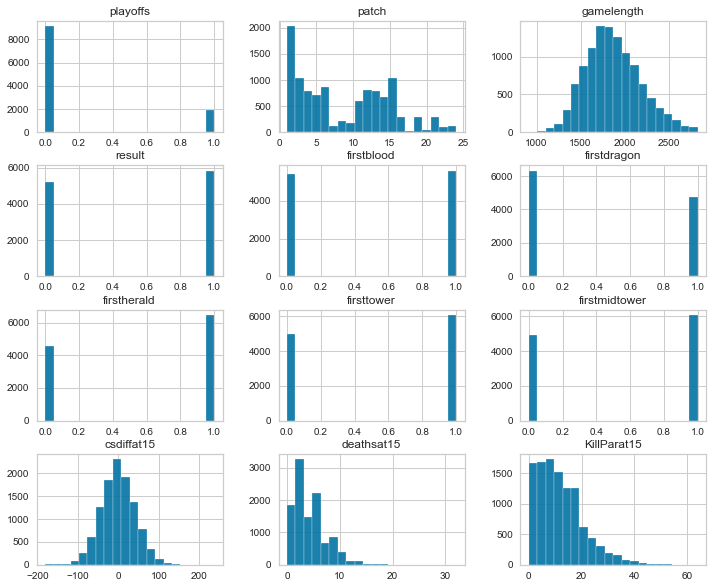
\includegraphics[width=1\textwidth]{figures/DistributionVisualisation}
    \caption{Graphs showing the distribution of data for the dataset}
    \label{fig:DistroVisual}
\end{figure}

\chapter{Feature Correlations}\label{ch:Feature Correlations}

\begin{figure}[h!]
    \centering
    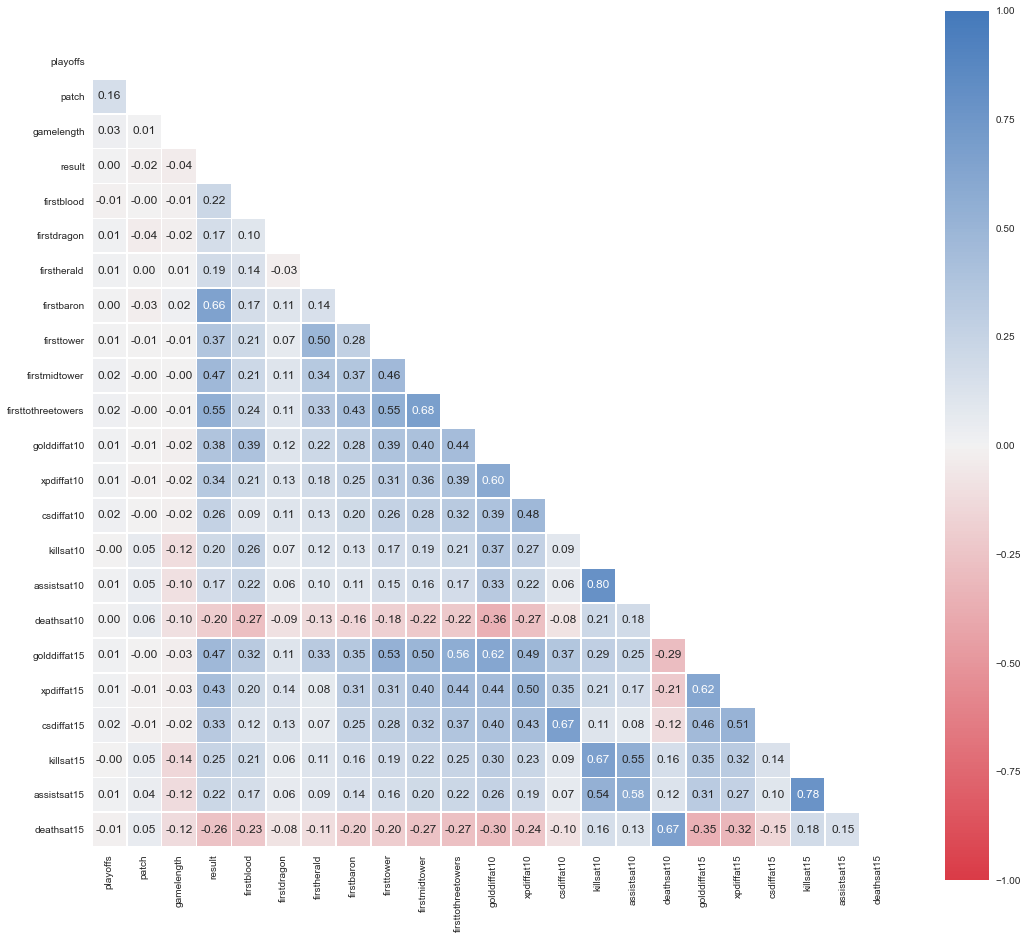
\includegraphics[width=1\textwidth]{figures/CorrMat1}
    \caption{A matrix of correlations between features in the dataset}
    \label{fig:CorrMat1}
\end{figure}

\begin{figure}[h!]
    \centering
    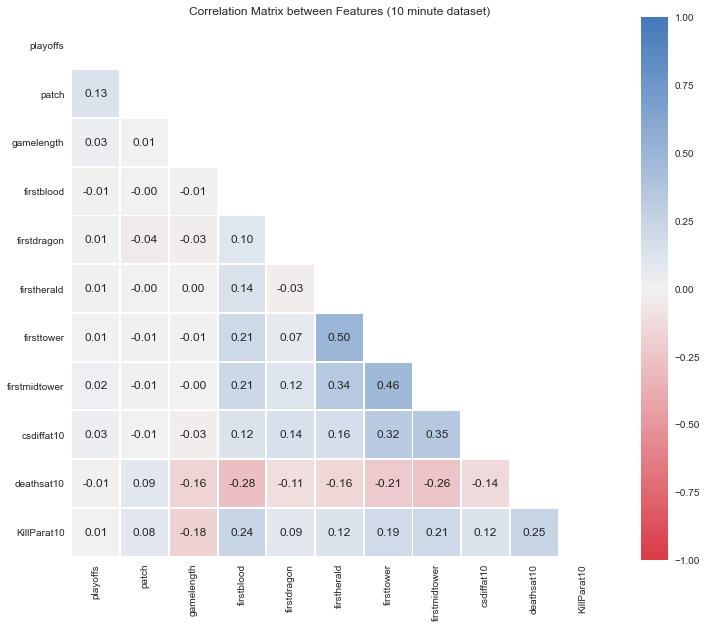
\includegraphics[width=1\textwidth]{figures/CorrMat10}
    \caption{A matrix of correlations from the 10-minute dataset}
    \label{fig:CorrMat10}
\end{figure}

\begin{figure}[h!]
    \centering
    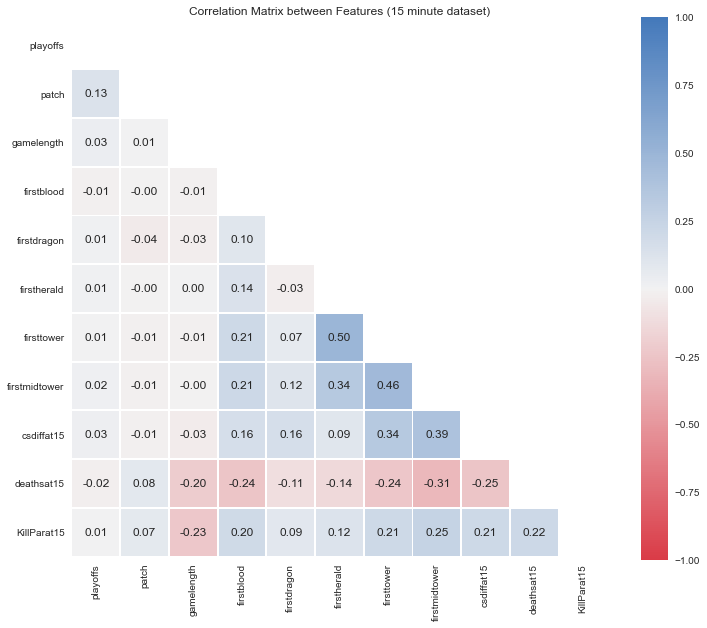
\includegraphics[width=1\textwidth]{figures/CorrMat15}
    \caption{A matrix of correlations from the 15-minute dataset}
    \label{fig:CorrMat15}
\end{figure}

\begin{figure}[h!]
    \centering
    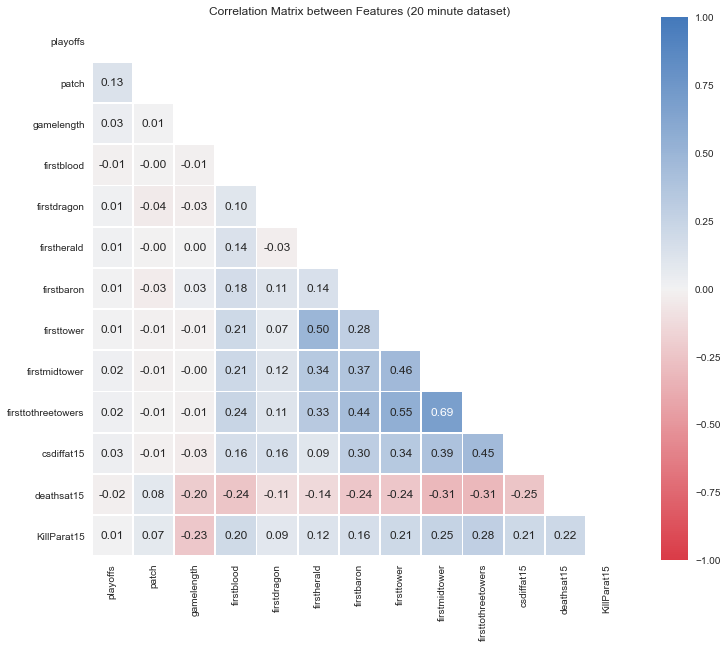
\includegraphics[width=1\textwidth]{figures/CorrMat20}
    \caption{A matrix of correlations from the 20-minute dataset}
    \label{fig:CorrMat20}
\end{figure}